Una risposta corretta, un'esecuzione priva di eccezioni e un servizio
raggiungibile sono proprietà distinte. Il livello di osservabilità permette di
esaminare le ultime due e di ricostruire il percorso che ha prodotto la prima;
la valutazione semantica è invece affidata ai riferimenti e ai controlli del
Capitolo~\ref{cap:7}. Questo capitolo descrive la strumentazione LLMOps del
prototipo, basata su Prometheus, Grafana e OpenTelemetry/Phoenix, e il modo in
cui i suoi dati vanno letti \cite{guidaProgetto2026}.

\section{Log, metriche e trace}

I log descrivono eventi puntuali, come un timeout o un nuovo tentativo. Le
metriche riassumono quantità numeriche nel tempo, come il numero di esecuzioni
e la distribuzione delle durate. Un trace collega le operazioni di una singola
richiesta: ciascuno span rappresenta un intervallo con i suoi attributi,
l'eventuale errore e la relazione con le operazioni che lo contengono
\cite{otelTraces}.

Le tre rappresentazioni rispondono a domande complementari. Un aumento delle
durate segnala un gruppo di richieste lente, il trace individua il passaggio
coinvolto e il log precisa l'errore. La correttezza del contenuto resta una
questione separata: una ricerca valida sulla città sbagliata termina
tecnicamente con successo.

\section{Architettura della telemetria}

Prometheus interroga il backend ogni 15 secondi e conserva le serie temporali
delle metriche; Grafana le presenta in dashboard. OpenTelemetry invia invece i
trace a Phoenix, che permette di esplorare il percorso di ogni richiesta e di
raggruppare le richieste di una stessa conversazione \cite{phoenixTracing}.
I due flussi sono rappresentati nella Figura~\ref{fig:telemetria}.

\begin{figure}[htbp]
\centering
\resizebox{0.96\textwidth}{!}{%
\begin{tikzpicture}[
    box/.style={rectangle,rounded corners,draw=blue!65!black,thick,
        fill=blue!8,align=center,minimum height=11mm,text width=34mm},
    line/.style={-{Latex[length=2mm]},thick}
]
    \node[box] (backend) at (0,0) {Backend strumentato};
    \node[box] (prom) at (5,1.7) {Prometheus\\serie temporali};
    \node[box] (graf) at (10,1.7) {Grafana\\viste aggregate};
    \node[box] (phoenix) at (5,-1.7) {Phoenix\\trace per richiesta};
    \draw[line] (prom) -- node[above left,font=\small]{GET /metrics} (backend);
    \draw[line] (graf) -- node[above,font=\scriptsize]{PromQL} (prom);
    \draw[line] (backend) -- node[below left,font=\small]{OTLP/HTTP} (phoenix);
\end{tikzpicture}}
\caption{Due flussi della telemetria: raccolta delle metriche in modalità
pull ed esportazione dei trace in modalità push. Le frecce indicano
l'iniziatore della richiesta o dell'invio.}
\label{fig:telemetria}
\end{figure}

\begin{figure}[htbp]
\centering
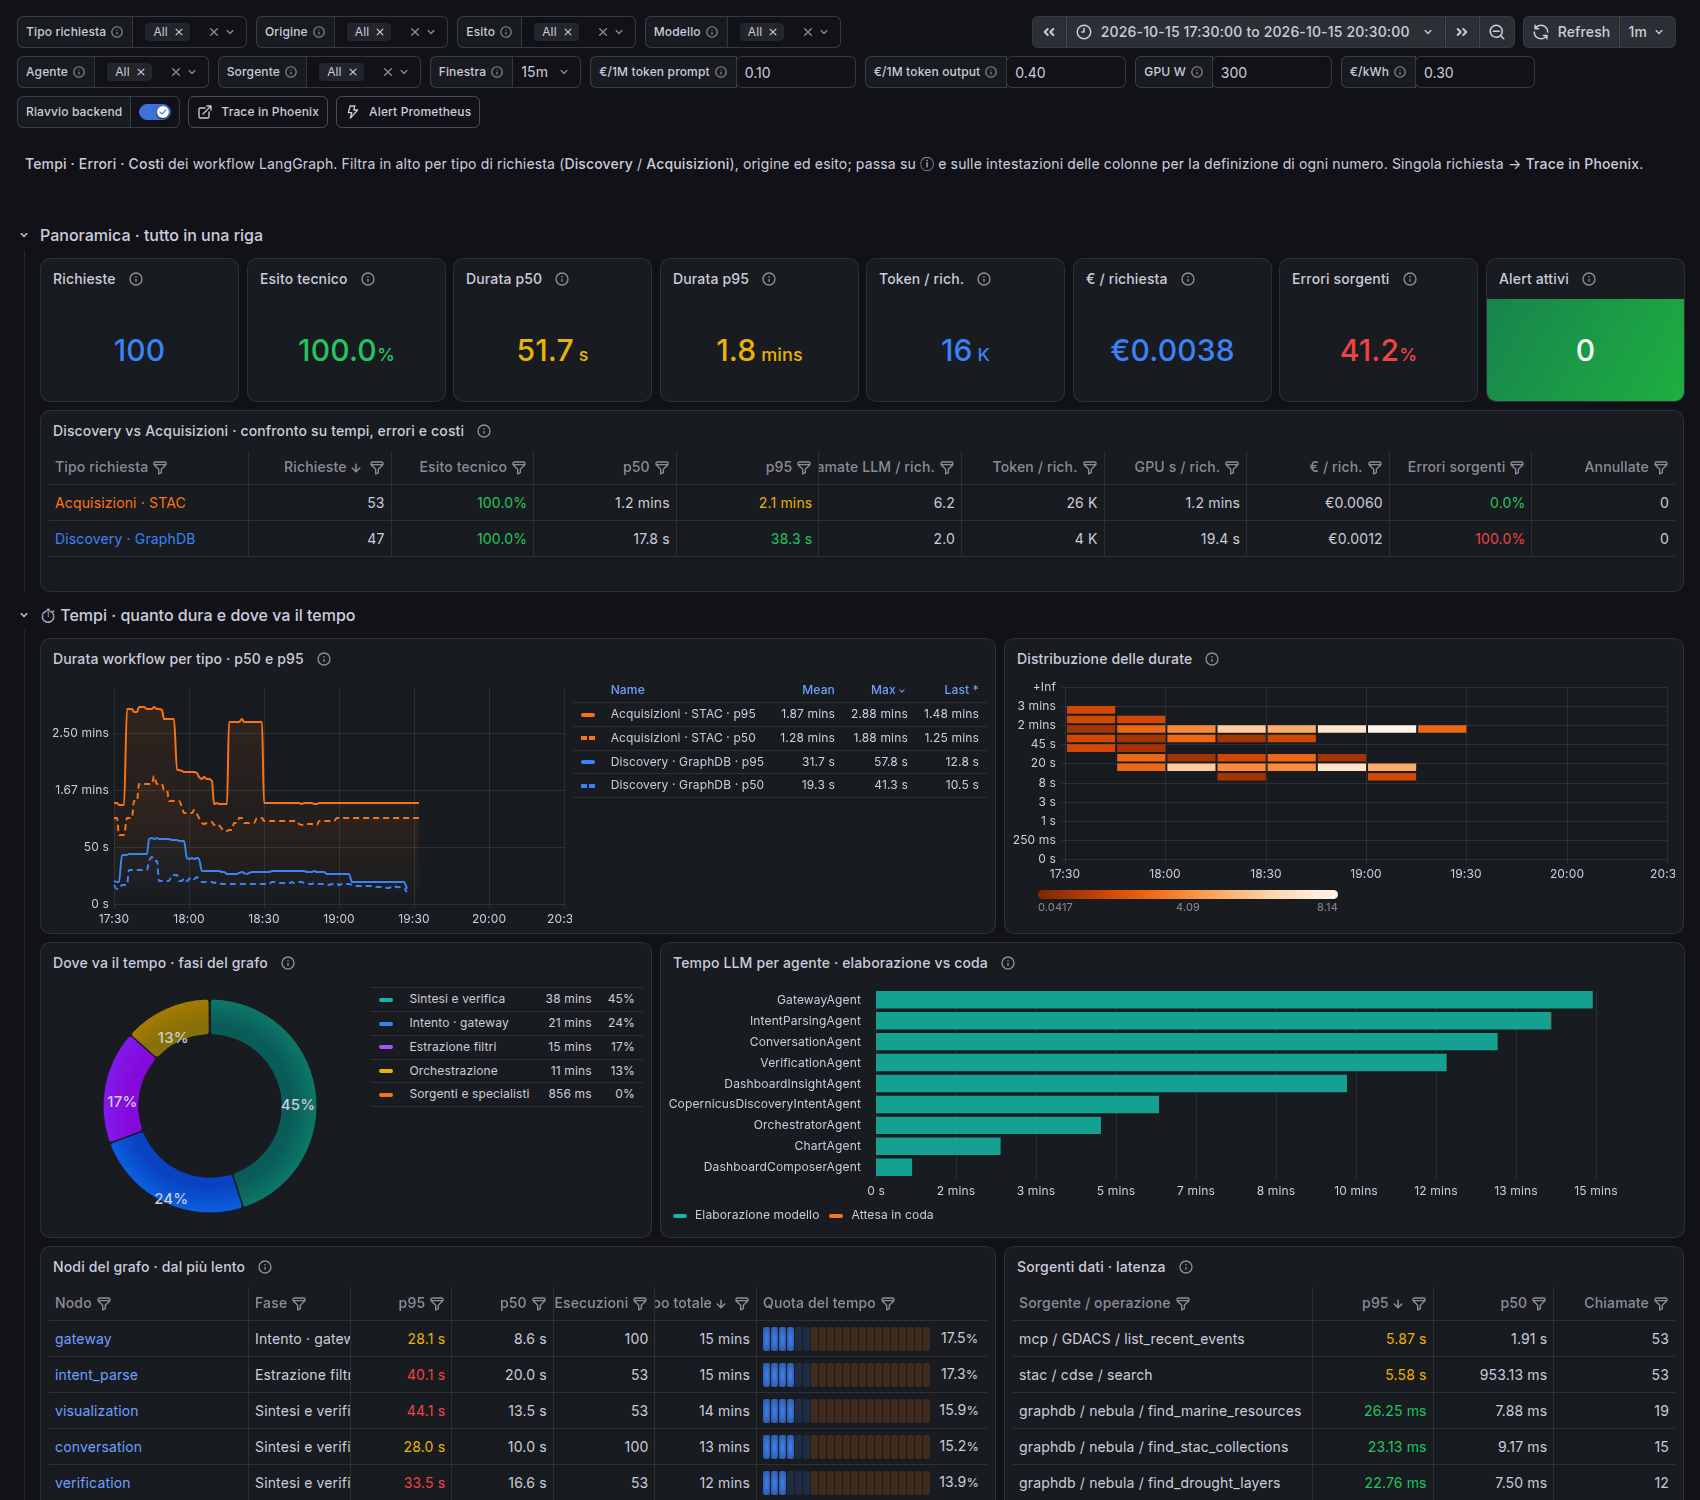
\includegraphics[width=0.95\textwidth]{Images/screenshots/grafana-llmops-live.png}
\caption{Dashboard Grafana \emph{Copernicus · LLMOps}: panoramica di richieste,
esiti, durate e confronto Discovery/acquisizioni, con collegamenti a Phoenix e
agli alert Prometheus.}
\label{fig:grafana-llmops}
\end{figure}

L'osservabilità si attiva come estensione opzionale del deployment e
strumenta la stessa applicazione, senza modificarne il codice. I dati sono
conservati per 15 giorni. I risultati del Judge restano nei propri file e
nella propria interfaccia, separati dalla telemetria operativa.

\section{Che cosa viene misurato}

La strumentazione avvolge le operazioni principali del backend, ne misura la
durata e ne registra l'esito. Copre quattro livelli.

\begin{itemize}
    \item \textbf{Richieste HTTP e chat.} Per ogni richiesta sono registrati
    stato e durata. Per la chat in streaming sono distinti il primo evento,
    il primo contenuto testuale e la conclusione, perché un aggiornamento di
    stato precede di solito la risposta vera e propria. L'esito finale
    distingue completamento, errore, interruzione e disconnessione del client.
    \item \textbf{Workflow e nodi.} Ogni esecuzione del workflow e ogni nodo
    del grafo producono uno span con durata, esito e stadio logico (intento,
    estrazione, orchestrazione, specialista, sintesi).
    \item \textbf{Strumenti e catalogo.} Sono tracciate le chiamate agli
    strumenti MCP e le query al catalogo a grafo, con il numero di risultati.
    \item \textbf{Chiamate al modello.} Per ciascuna invocazione sono separati
    il tempo d'attesa in coda, il tempo di inferenza e gli eventuali nuovi
    tentativi; sono registrati anche i token in ingresso e in uscita forniti
    dal server del modello \cite{ollamaUsage}, da cui si ricava la velocità di
    generazione in token al secondo.
\end{itemize}

Il conteggio dei token rappresenta il consumo registrato dalle chiamate
osservate, utile per confrontare agenti e periodi; il Judge usa un canale
proprio ed è escluso da questo conteggio. Le durate degli span sono annidate:
il tempo di un nodo è già compreso in quello del workflow che lo contiene.

\section{Come leggere le metriche}

Prometheus usa tre tipi di misura: i contatori, che crescono nel tempo (per
esempio il numero di richieste); i gauge, che indicano un valore corrente (per
esempio le chiamate in corso); gli istogrammi, che raggruppano le durate in
fasce e permettono di stimarne la distribuzione \cite{prometheusHistograms}.
I valori per periodo mostrati in dashboard sono stime ricavate da queste serie.

Per le durate la dashboard riporta due percentili. Il p50, o mediana, è la
durata entro cui si conclude metà delle richieste. Il p95 è la durata entro cui
si conclude il 95\% delle richieste: descrive le richieste più lente senza
farsi dominare da un singolo caso estremo. È quindi un indicatore di
reattività, distinto sia dalla durata massima sia dalla qualità della risposta,
e diventa affidabile quando il numero di campioni è sufficiente.

La dashboard calcola due tassi di successo su popolazioni diverse:
\[
 r_{\mathrm{workflow}} =
 \frac{N_{\mathrm{ok}}}{N_{\mathrm{ok}}+N_{\mathrm{error}}},
 \qquad
 r_{\mathrm{chat}} =
 \frac{N_{\mathrm{completed}}}
 {N_{\mathrm{completed}}+N_{\mathrm{error}}+N_{\mathrm{interrupted}}}.
\]
Il primo esclude le esecuzioni annullate, il secondo le disconnessioni del
client; entrambi vanno letti insieme alle tabelle degli esiti. In assenza di
traffico il rapporto resta vuoto, condizione distinta da un tasso pari a zero.

\section{Dashboard Grafana e alert}

La dashboard è generata da uno script e caricata automaticamente all'avvio
\cite{grafanaProvisioning}: la versione nel repository è quella di
riferimento. È organizzata in sezioni tematiche, riassunte nella
Tabella~\ref{tab:viste-osservabilita}, e include una guida espandibile che
spiega unità di misura, percentili, token ed esiti.

\begin{table}[htbp]
\centering
\small
\begin{tabularx}{\textwidth}{>{\bfseries\raggedright\arraybackslash}p{0.25\textwidth}
    >{\raggedright\arraybackslash}X}
\toprule
Sezione & Domanda a cui risponde \\
\midrule
Panoramica & Il sistema sta raccogliendo dati? Quante richieste riescono e in
quanto tempo? \\
\addlinespace
Diagnosi & Da dove vengono gli errori? Quali nodi e servizi esterni sono più
lenti? \\
\addlinespace
LLM & Quante chiamate al modello sono attive o in coda? Quanti tentativi e
quanti token per agente? \\
\addlinespace
Chat & Quanto tempo passa prima della prima risposta? Come si concludono le
conversazioni? \\
\addlinespace
HTTP e stadi & Quanto traffico riceve ogni servizio e quanti errori del
server produce? \\
\bottomrule
\end{tabularx}
\caption{Sezioni principali della dashboard, affiancate dalla guida alle metriche.}
\label{tab:viste-osservabilita}
\end{table}

I filtri permettono di restringere le viste per tipo di richiesta, esito,
modello o agente (Figura~\ref{fig:grafana-filtri}); la sezione dedicata al
modello è mostrata nella Figura~\ref{fig:grafana-llm}. Prima di leggere uno
storico conviene controllare l'indicatore di raccolta, che segnala se i dati
sono aggiornati.

\begin{figure}[htbp]
\centering
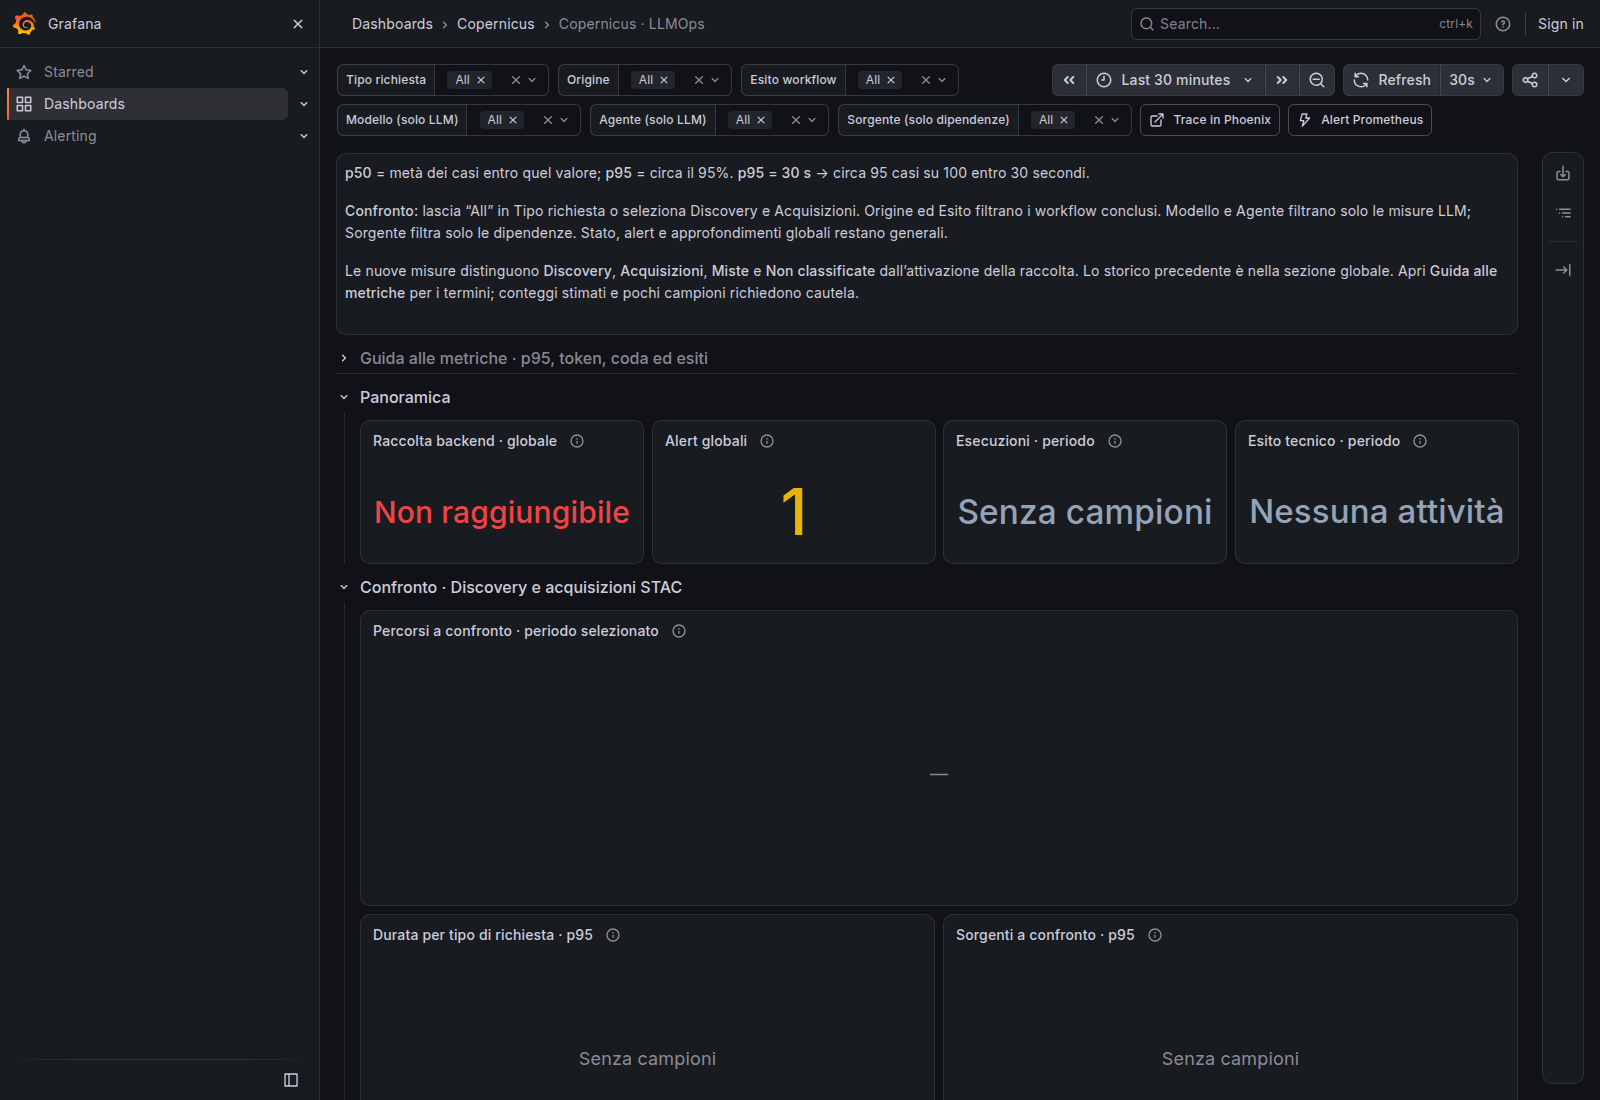
\includegraphics[width=0.95\textwidth]{Images/screenshots/ui-filtri-panoramica.png}
\caption{Filtri della dashboard LLMOps (tipo richiesta, origine, esito,
modello, agente, sorgente) e riga di panoramica con stato della raccolta e
alert.}
\label{fig:grafana-filtri}
\end{figure}

\begin{figure}[htbp]
\centering
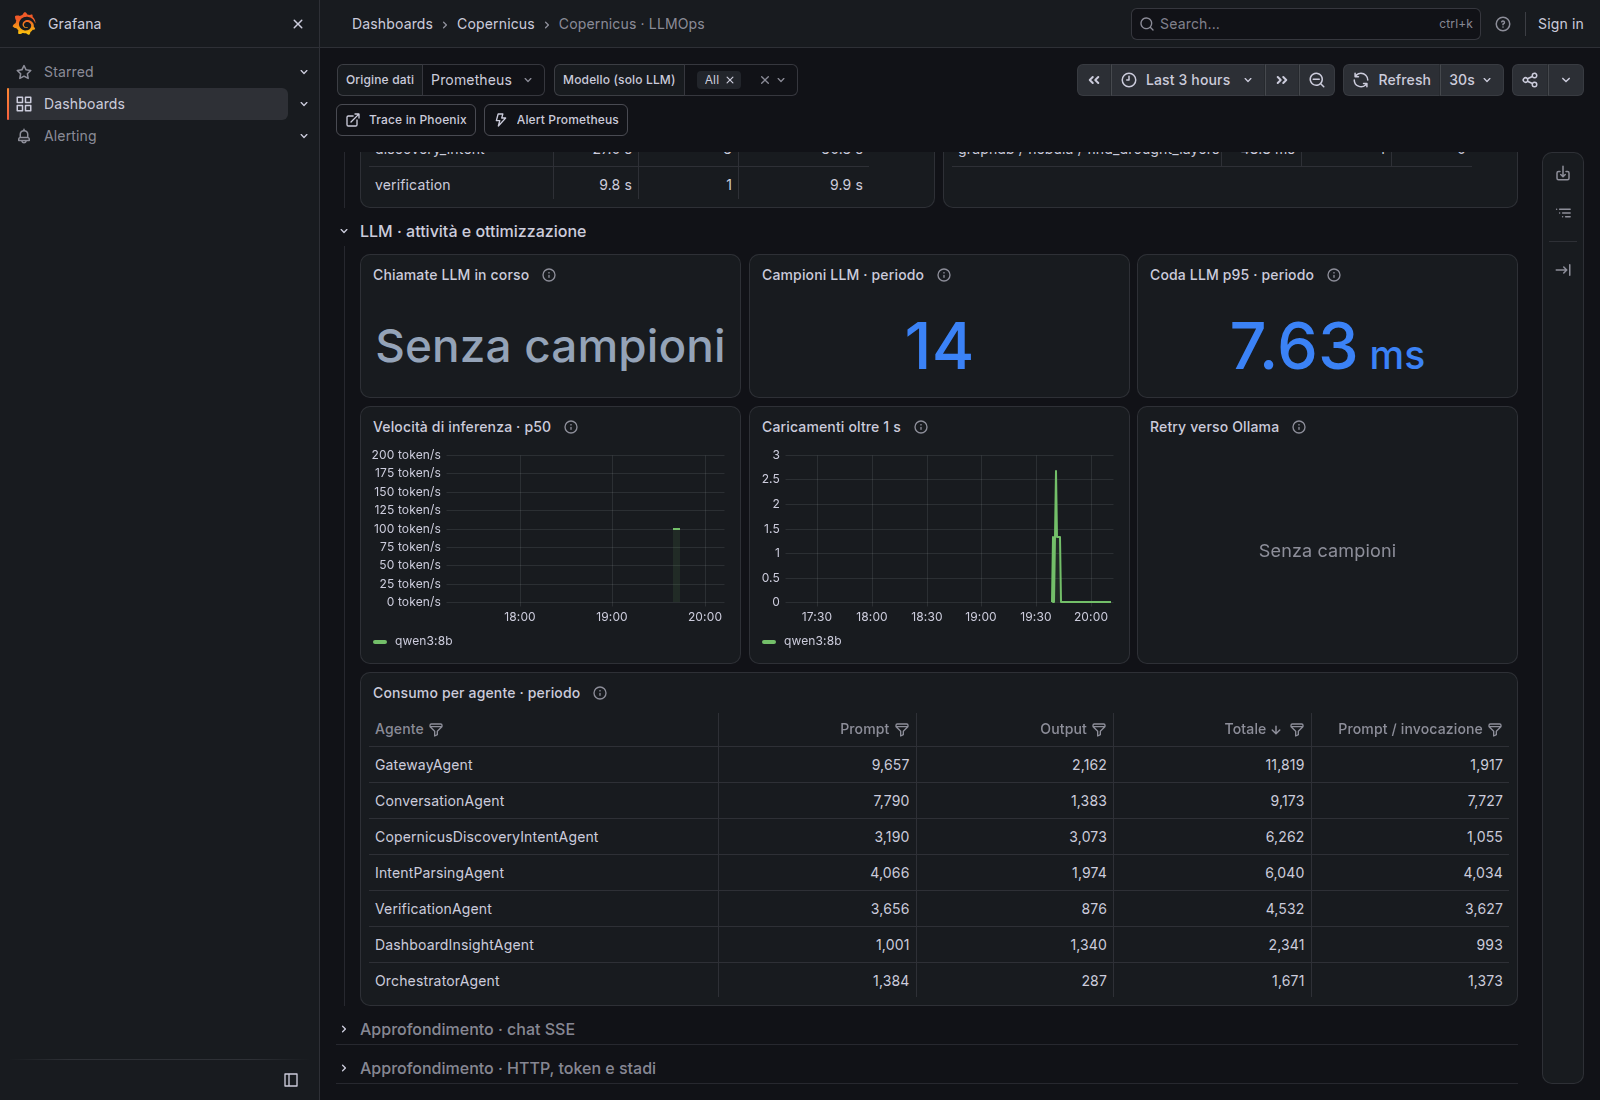
\includegraphics[width=0.95\textwidth]{Images/screenshots/grafana-llm.png}
\caption{Sezione LLM della stessa dashboard: coda, retry, token per agente e
salute delle invocazioni al modello.}
\label{fig:grafana-llm}
\end{figure}

Le regole di alert coprono backend irraggiungibile, errori HTTP, stream
falliti, prima risposta lenta, coda del modello e guasti degli strumenti. Un
alert scatta quando la condizione persiste per un intervallo prefissato. Gli
alert sono visibili in Prometheus e in Grafana; nel prototipo manca un canale
di notifica verso persone o sistemi esterni.

\section{Diagnosi e copertura}

Quando una richiesta è lenta, il percorso di analisi parte dalla panoramica
(raccolta attiva, numero di campioni) e scende verso workflow, nodi, coda del
modello, tentativi e servizi esterni. Una coda lunga con inferenza stabile
indica attesa per il modello; un nodo lento con chiamate al modello brevi
orienta verso altri passaggi. Il trace della richiesta conferma l'ipotesi
mostrando dove si concentra il tempo, e i log precisano gli errori.

Quando una risposta è sbagliata, il confronto riguarda domanda, luogo
interpretato, query, record restituiti e artefatto finale. Qui gli indicatori
tecnici possono risultare tutti positivi: la verifica del contenuto spetta al
benchmark e, per tabella e mappa, a una prova dell'interfaccia.

La copertura riguarda tempi, esiti e consumo di token. Restano fuori l'uso
della GPU, le risorse dei singoli container e l'accuratezza semantica; alcune
dipendenze, come il catalogo STAC, la ricerca web e il Judge, compaiono solo
attraverso il tempo del nodo che le invoca. I trace possono inoltre registrare
prompt e risposte: la cattura del contenuto è configurabile e limitata in
lunghezza, ma va considerata un dato potenzialmente sensibile.

La ricognizione del 15 ottobre 2026 illustra questi aspetti: Grafana mostrava
ancora i dati storici mentre Prometheus segnalava il backend irraggiungibile,
con l'alert corrispondente attivo \cite{guidaProgetto2026}. La presenza di
grafici, la salute corrente del servizio e la correttezza dei risultati vanno
quindi verificate separatamente.
